\documentclass[11pt]{article}
\usepackage{amssymb}
\usepackage{amsthm}
\usepackage{enumitem}
\usepackage{physics,amsmath}
\usepackage{bm}
\usepackage{adjustbox}
\usepackage{mathrsfs}
\usepackage{graphicx}
\usepackage{siunitx}
\usepackage[mathscr]{euscript}


\title{\textbf{Solved selected problems of General Relativity - Thomas A. Moore}}
\author{Franco Zacco}
\date{}

\addtolength{\topmargin}{-3cm}
\addtolength{\textheight}{3cm}

\newcommand{\hatr}{\bm{\hat{r}}}
\newcommand{\hatn}{\bm{\hat{n}}}
\newcommand{\hatx}{\bm{\hat{x}}}
\newcommand{\haty}{\bm{\hat{y}}}
\newcommand{\hatz}{\bm{\hat{z}}}
\newcommand{\hatth}{\bm{\hat{\theta}}}
\newcommand{\hatphi}{\bm{\hat{\phi}}}
\newcommand{\hatrho}{\bm{\hat{\rho}}}
\newcommand{\er}{\bm{e}_r}
\newcommand{\etht}{\bm{e}_\theta}

\theoremstyle{definition}
\newtheorem*{solution*}{Solution}
\renewcommand*{\proofname}{Solution}

\begin{document}
\maketitle
\thispagestyle{empty}

\section*{Chapter 11 - Precession of the perihelion}

\begin{proof}{\textbf{BOX 11.1} - Exercise 11.1.1.}\\
    From equation (11.5) we know that
    \begin{align*}
        u = \frac{1}{r} \quad\quad \dv{r}{\phi} = -\frac{1}{u^2}\dv{u}{\phi} 
    \end{align*}
    Replacing these values in equation (11.6) we get that 
    \begin{align*}
        \tilde{E} &= \frac{1}{2}\left(\dv{r}{\phi}\right)^2\frac{l^2}{r^4}
        - \frac{GM}{r} + \frac{l^2}{2r^2} - \frac{GMl^2}{r^3}\\
        2\tilde{E} &= \left(\dv{u}{\phi}\right)^2l^2 - 2GMu + u^2l^2 - 2GMl^2u^3
    \end{align*}
    Now taking the derivative with respect to $\phi$ we have that
    \begin{align*}
        0 &= 2l^2\dv{u}{\phi}\dv[2]{u}{\phi}
        - 2GM\dv{u}{\phi} + 2l^2u\dv{u}{\phi} - 6GMl^2u^2\dv{u}{\phi}\\
        0 &= 2l^2\dv[2]{u}{\phi} - 2GM + 2l^2u - 6GMl^2u^2\\
        0 &= \dv[2]{u}{\phi} - \frac{GM}{l^2} + u - 3GMu^2
    \end{align*}
    Therefore
    \begin{align*}
        \dv[2]{u}{\phi} + u &= \frac{GM}{l^2} + 3GMu^2
    \end{align*}
\end{proof}
\cleardoublepage
\begin{proof}{\textbf{BOX 11.2} - Exercise 11.2.1.}\\
    First let us note that
    \begin{align*}
        \dv{r}{t} = \dv{r}{\phi}\dv{\phi}{t} = \dv{r}{\phi}\frac{l}{r^2}
    \end{align*}
    where we used that $d\phi/dt = l/r^2$ from (11.20). In the same way as in
    (11.5) we can replace $r$ with $u$ using the following equations 
    \begin{align*}
        u = \frac{1}{r} \qquad \dv{r}{\phi} = -\frac{1}{u^2}\dv{u}{\phi}
    \end{align*}
    Then equation (11.20) becomes
    \begin{align*}
        \tilde{E}_N &= \frac{1}{2}\left(\dv{r}{\phi}\right)^2\frac{l^2}{r^4}
        - \frac{GM}{r} + \frac{l^2}{2r^2}\\
        2\tilde{E}_N &= \left(\dv{u}{\phi}\right)^2l^2 - 2GMu + l^2u^2
    \end{align*}
    Now taking the derivative with respect to $\phi$ we have that
    \begin{align*}
        0 &= 2l^2\dv{u}{\phi}\dv[2]{u}{\phi}
        - 2GM\dv{u}{\phi} + 2l^2u\dv{u}{\phi}\\
        0 &= 2l^2\dv[2]{u}{\phi} - 2GM + 2l^2u\\
        0 &= \dv[2]{u}{\phi} - \frac{GM}{l^2} + u
    \end{align*}
    Therefore
    \begin{align*}
        \dv[2]{u}{\phi} + u &= \frac{GM}{l^2}
    \end{align*}
\end{proof}
\cleardoublepage
\begin{proof}{\textbf{BOX 11.3} - Exercise 11.3.1.}\\
    Equation (11.6) states that
    \begin{align*}
        \dv[2]{u}{\phi} + u = \frac{GM}{l^2} + 3GMu^2
    \end{align*}
    But if we consider an almost circular orbit then $r$ is going to be constant
    and hence $u$ too so $du/d\phi \approx 0$ hence we can write that
    \begin{align*}
        u_c = \frac{GM}{l^2} + 3GMu_c^2
    \end{align*}
    Now, if we consider a perturbation of this orbit
    $u(\phi) = u_c + u_cw(\phi)$ and we replace this value in equation (11.6)
    we get that
    \begin{align*}
        \dv[2]{\phi}(u_c + u_cw) + u_c + u_cw
        &= \frac{GM}{l^2} + 3GM(u_c + u_cw)^2\\
        \dv[2]{u_c}{\phi} + u_c\dv[2]{w}{\phi} 
        + 2 \dv{u_c}{\phi}\dv{w}{\phi} + w\dv[2]{u_c}{\phi}
        + u_c + u_cw &= \frac{GM}{l^2} + 3GM(u_c + u_cw)^2\\
        u_c\dv[2]{w}{\phi} + u_c + u_cw
        &= \frac{GM}{l^2} + 3GM(u_c + u_cw)^2
    \end{align*}
    Where we used again that $du_c/d\phi \approx 0$.
    Expanding the equation and replacing the value we have for $u_c$ we get
    that
    \begin{align*}
        u_c\dv[2]{w}{\phi} + \frac{GM}{l^2} + 3GMu_c^2 + u_cw
        &= \frac{GM}{l^2} + 3GMu_c^2 + 6GMu_c^2w + 3GMu_c^2w^2\\
        u_c\dv[2]{w}{\phi} + u_cw &= 6GMu_c^2w + 3GMu_c^2w^2\\
        \dv[2]{w}{\phi} + w &= 6GMu_cw + 3GMu_cw^2
    \end{align*}
\end{proof}
\begin{proof}{\textbf{BOX 11.4} - Exercise 11.4.1.}\\
    The predicted perihelion shift is given by
    $6\pi GM/r_c$.
    Hence replacing values we have that
    \begin{align*}
        \frac{6\pi\cdot 1.477}{57.9\times 10^6} 
        = 4.808\times 10^{-7}~\text{radians} 
    \end{align*}
    This is the shift predicted for each period of 0.241 years so in 100 years
    will be 
    \begin{align*}
        4.808\times 10^{-7} \cdot \frac{100}{0.241}
        = 0.0001995~\text{radians/century}
    \end{align*}
    Equivalently in arc-second this is
    \begin{align*}
        0.0001995\cdot \frac{180}{\pi} \cdot 3600
        = 41.15~\text{arc-second/century}
    \end{align*}
\end{proof}
\cleardoublepage
\begin{proof}{\textbf{BOX 11.5} - Exercise 11.5.1.}\\
    From equation (11.23) we have that
    \begin{align*}
        1 + \left(\dv{z}{r}\right)^2 &= \frac{1}{1 - 2GM/r}\\
        \dv{z}{r} &= \sqrt{\frac{1}{1 - 2GM/r} - 1}\\
        \dv{z}{r} &= \sqrt{\frac{2GM}{r - 2GM}}
    \end{align*}
    Then by integrating we get that
    \begin{align*}
        \int dz &= \int \sqrt{\frac{2GM}{r - 2GM}} dr\\
        z &= \sqrt{8GM(r - 2GM)} + C
    \end{align*}
\end{proof}
\begin{proof}{\textbf{BOX 11.6} - Exercise 11.6.1.}\\
    Let $\alpha$ be small then we can approximate $\tan\alpha \approx \alpha$
    and $\cos\alpha \approx 1 - \frac{1}{2}\alpha^2$ then equation 11.16
    becomes
    \begin{align*}
        2\pi - \delta &= 2\pi \left(1 - \frac{1}{2}\alpha^2\right)\\
        \delta &= \pi\alpha^2
    \end{align*}
    Also, by this approximation we know that $\alpha = \dv{z}{r}$ and by
    differentiation of $z(r)$ we get that
    \begin{align*}
        \alpha = \dv{z}{r} = \sqrt{\frac{2GM}{r - 2GM}}
    \end{align*}
    But since we are assuming that $r \gg 2GM$ we can approximate $\alpha$ as   
    \begin{align*}
        \alpha = \sqrt{\frac{2GM}{r}}
    \end{align*}
    Therefore replacing the value of $\alpha$ we get that
    \begin{align*}
        \delta &= \frac{2\pi GM}{r}
    \end{align*}
\end{proof}
\cleardoublepage
\begin{proof}{\textbf{BOX 11.7} - Exercise 11.7.1.}\\
    From equations (11.29a) and (11.29b) lets compute
    $\frac{1}{2}(r_{n+1} + r_n)$ by adding both equation and multiplying by
    $1/2$ then
    \begin{align*}
        r_{n+1} + r_n &= \left[r_{n+1/2}
        + \underset{\text{at }\tau_{n + 1/2}}{\left[\dv{r}{\tau}\right]}
        \frac{1}{2}\Delta\tau
        + \frac{1}{2}
        \underset{\text{at }\tau_{n + 1/2}}{\left[\dv[2]{r}{\tau}\right]}
        (\frac{1}{2}\Delta\tau)^2
        + O(\Delta\tau^3)
        \right]\\
        &\quad + \left[r_{n+1/2}
        - \underset{\text{at }\tau_{n + 1/2}}{\left[\dv{r}{\tau}\right]}
        \frac{1}{2}\Delta\tau
        + \frac{1}{2}
        \underset{\text{at }\tau_{n + 1/2}}{\left[\dv[2]{r}{\tau}\right]}
        (\frac{1}{2}\Delta\tau)^2
        - O(\Delta\tau^3)
        \right]\\
        r_{n+1} + r_n &= 2r_{n+1/2}
        + \underset{\text{at }\tau_{n + 1/2}}{\left[\dv[2]{r}{\tau}\right]}
        (\frac{1}{2}\Delta\tau)^2\\
        \frac{1}{2}(r_{n+1} + r_n) &= r_{n+1/2}
        + \frac{1}{2}
        \underset{\text{at }\tau_{n + 1/2}}{\left[\dv[2]{r}{\tau}\right]}
        \frac{1}{4}\Delta\tau^2
    \end{align*}
    This implies that $\frac{1}{2}(r_{n+1} + r_n)$ is a second-order-accurate
    approximation for $r_{n+1/2}$.

    Now, let us compute $\phi_{n+1} - \phi_n$ using equations (11.29c) and
    (11.29d) then
    \begin{align*}
        \phi_{n+1} - \phi_n &= \left[\phi_{n+1/2}
        + \underset{\text{at }\tau_{n + 1/2}}{\left[\dv{\phi}{\tau}\right]}
        \frac{1}{2}\Delta\tau
        + \frac{1}{2}
        \underset{\text{at }\tau_{n + 1/2}}{\left[\dv[2]{\phi}{\tau}\right]}
        (\frac{1}{2}\Delta\tau)^2
        + O(\Delta\tau^3)
        \right]\\
        &\quad - \left[\phi_{n+1/2}
        - \underset{\text{at }\tau_{n + 1/2}}{\left[\dv{\phi}{\tau}\right]}
        \frac{1}{2}\Delta\tau
        + \frac{1}{2}
        \underset{\text{at }\tau_{n + 1/2}}{\left[\dv[2]{\phi}{\tau}\right]}
        (\frac{1}{2}\Delta\tau)^2
        - O(\Delta\tau^3)
        \right]\\
        \phi_{n+1} - \phi_n &= 
        \underset{\text{at }\tau_{n + 1/2}}{\left[\dv{\phi}{\tau}\right]}
        \Delta\tau + 2O(\Delta\tau^3)
    \end{align*}
    Therefore $\phi_{n+1} - \phi_n$ is a second-order-accurate approximation
    for $[d\phi/d\tau]\Delta \tau$ evaluated at $\tau_{n+1/2}$.
\end{proof}
\cleardoublepage
\begin{proof}{\textbf{BOX 11.7} - Exercise 11.7.2.}\\
    Let us take equation (11.24) when $d^2r_c/d\tau^2 = 0$ then solving for
    $l$ gives us
    \begin{align*}
        0 &= -\frac{GM}{r_c^2} + \frac{l_c^2}{r_c^3} - \frac{3GMl_c^2}{r_c^4}\\
        l_c^2\left[\frac{1}{r_c^3} - \frac{3GM}{r_c^4}\right] &=
        \frac{GM}{r_c^2}\\
        l_c^2 &=
        \frac{GM}{r_c^2}\left[\frac{r_c^4}{r_c - 3GM}\right]\\
        l_c^2 &=\frac{r_c^2}{r_c/GM - 3}\\
        \frac{l_c}{GM} &=\frac{r_c/GM}{\sqrt{r_c/GM - 3}}
    \end{align*} 
\end{proof}
\begin{proof}{\textbf{P11.1}}
    We know that the equation to compute the perihelion shift is
    $$\frac{6\pi GM}{r_c}$$
    So this implies a perihelion shift for Venus of
    \begin{align*}
        \Delta\phi_V = \frac{6\pi \cdot 1.477}{108.2 \times 10^6}
        = 2.573\times 10^{-7}~\text{radians}
    \end{align*}
    This is the shift predicted for each period of 0.615 years so in 100 years
    will be
    \begin{align*}
        2.573\times 10^{-7}\cdot \frac{100}{0.615}\cdot\frac{180}{\pi}\cdot3600
        = 8.62~\text{arcseconds/century}
    \end{align*}
    In the same way for the Earth and Mars we have that
    \begin{align*}
        \Delta\phi_E = \frac{6\pi \cdot 1.477}{149.6 \times 10^6}
        = 1.861\times 10^{-7}~\text{radians}\\
        \Delta\phi_M = \frac{6\pi \cdot 1.477}{227.9 \times 10^6}
        = 1.221\times 10^{-7}~\text{radians}
    \end{align*}
    And hence
    \begin{align*}
        1.861\times 10^{-7}\cdot \frac{100}{1}\cdot\frac{180}{\pi}\cdot3600
        &= 3.838~\text{arcseconds/century}\\
        1.221\times 10^{-7}\cdot \frac{100}{1.881}\cdot\frac{180}{\pi}\cdot3600
        &= 1.339~\text{arcseconds/century}
    \end{align*}
\end{proof}
\cleardoublepage
\begin{proof}{\textbf{P11.3}}
    We know that the equation to compute the periastron shift is
    $$\Delta\phi = \frac{6\pi GM}{r_c}$$
    So in this case we have that
    \begin{align*}
        \Delta\phi = \frac{6\pi \cdot 2.0}{400}
        = 0.09424~\text{radians} = 5.3995^\circ
    \end{align*}
    For someone at infinity the period of the orbit is given by Kepler's law 
    derived in the previous chapter as
    \begin{align*}
        T = \frac{2\pi}{\sqrt{GM}}\sqrt{r^3}
        = \frac{2\pi}{\sqrt{2}}~\sqrt{400^3}
        = 35543.0635~km = 0.1185~s
    \end{align*}
    Therefore the precession rate is
    \begin{align*}
        \frac{\Delta \phi}{T} = \frac{5.3995}{0.1185} = 45.56~^\circ/s 
    \end{align*}
\end{proof}
\cleardoublepage
\begin{proof}{\textbf{P11.5}}
Let a spacetime metric given by
\begin{align*}
    ds^2 = -\left(1 - \frac{2GM}{r}\right)dt^2 + dr^2 + r^2d\theta^2
    + r^2\sin^2\theta d\phi^2
\end{align*}
\begin{itemize}
    \item [\textbf{a.}] Let $\mu = t$ then since the metric is both diagonal
    and time-independent then equation 10.1 becomes
    \begin{align*}
        0 = \dv{\tau}(g_{tt}\dv{t}{\tau}) + 0
    \end{align*}
    Then $-g_{tt}\dv{t}{\tau} = e$ where $e$ is a constant, hence
    \begin{align*}
        \left(1 - \frac{2GM}{r}\right)\dv{t}{\tau} = e
    \end{align*}
    On the other hand, if $\mu = \phi$ as in Schwarzchild metric, our metric is
    both diagonal and independent of $\phi$ so we have that
    $g_{\phi\phi}\dv{\phi}{\tau} = l$ where $l$ is a constant then
    \begin{align*}
        r^2\sin^2\theta\dv{\phi}{\tau} = l
    \end{align*}
    Which implies that for the equatorial plane $\dv{\phi}{\tau} = l/r^2$.
    \item [\textbf{b.}] Let us compute $\bm{u}\cdot\bm{u} = -1$ as follows
    \begin{align*}
        -1 &= \bm{u}\cdot\bm{u}\\
        -1 &= -\left(1 - \frac{2GM}{r}\right)\left(\dv{t}{\tau}\right)^2
        + \left(\dv{r}{\tau}\right)^2
        + r^2\left(\dv{\theta}{\tau}\right)^2
        + r^2\sin^2\theta \left(\dv{\phi}{\tau}\right)^2\\
        -1 &= -\left(1 - \frac{2GM}{r}\right)\left(\dv{t}{\tau}\right)^2
        + \left(\dv{r}{\tau}\right)^2
        + r^2 \left(\dv{\phi}{\tau}\right)^2\\
        1 &= \left(1 - \frac{2GM}{r}\right)^{-1}e^2
        - \left(\dv{r}{\tau}\right)^2
        - \frac{l^2}{r^2}
    \end{align*}
    Where we used that the plane is equatorial i.e. $\theta = \pi/2$ but also
    $d\theta/d\tau = 0$ and we replaced the constants we got from $\textbf{a.}$
    \item [\textbf{c.}] First, let us note that
    \begin{align*}
        \dv{r}{\tau} = \dv{r}{\phi}\dv{\phi}{\tau} = \dv{r}{\phi}\frac{l}{r^2}
    \end{align*}
    Then the equation we determined in $\textbf{b.}$ becomes
    \begin{align*}
        1 &= \left(1 - \frac{2GM}{r}\right)^{-1}e^2
        - \left(\dv{r}{\phi}\right)^2\frac{l^2}{r^4}
        - \frac{l^2}{r^2}
    \end{align*}
    Now replacing $u = 1/r$ and $dr/d\phi = -r^2 du/d\phi = -(1/u^2)du/d\phi$
    we get that
    \begin{align*}
        1 &= \frac{e^2}{1 - 2GMu} - \left(\dv{u}{\phi}\right)^2l^2 - u^2 l^2
    \end{align*}
    Taking the derivative with respect to $\phi$ we see that
    \begin{align*}
        0 &= \frac{2e^2GM}{(1 - 2GMu)^2}\dv{u}{\phi}
        - 2l^2\dv{u}{\phi}\dv[2]{u}{\phi} - 2l^2u\dv{u}{\phi}\\
        0 &= \frac{2e^2GM}{(1 - 2GMu)^2} - 2l^2\dv[2]{u}{\phi} - 2l^2u\\
        \dv[2]{u}{\phi} + u &= \frac{e^2GM}{l^2(1 - 2GMu)^2}
    \end{align*}
    \item [\textbf{d.}]
    Applying the binomial approximation on $(1 - 2GMu)^{-2}$ we get that
    \begin{align*}
        \dv[2]{u}{\phi} + u &= \frac{e^2GM}{l^2}(1 + 4GMu)\\
        \dv[2]{u}{\phi} + u &= \frac{e^2GM}{l^2} + 4\left(\frac{eGM}{l}\right)^2u\\
        \dv[2]{u}{\phi} + \left[1 - 4\left(\frac{eGM}{l}\right)^2\right]u
        &= \frac{e^2GM}{l^2}
    \end{align*}
    \item [\textbf{e.}] Taking $u = u_c = \text{constant}$ equation 11.37
    becomes
    \begin{align*}
        \left[1 - 4\left(\frac{eGM}{l}\right)^2\right]u_c &= \frac{e^2GM}{l^2}
    \end{align*}
    Solving this equation for $(\frac{eGM}{l})^2$ we get that
    \begin{align*}
        u_c - 4u_c\left(\frac{eGM}{l}\right)^2
        &= \left(\frac{eGM}{l}\right)^2\frac{1}{GM}\\
        4u_c\left(\frac{eGM}{l}\right)^2 + \left(\frac{eGM}{l}\right)^2\frac{1}{GM}
        &= u_c\\
        \left(\frac{eGM}{l}\right)^2
        &= u_c\left(4u_c + \frac{1}{GM}\right)^{-1}\\
        \left(\frac{eGM}{l}\right)^2 &= \frac{u_c GM}{4u_cGM + 1}
    \end{align*}
\cleardoublepage
    \item [\textbf{f.}] Let us plug in the equation $u(\phi) = u_c + u_c w(\phi)$
    in the equation 11.37 then
    \begin{align*}
        u_c\dv[2]{w}{\phi}
        + \left[1 - 4\left(\frac{eGM}{l}\right)^2\right](u_c + u_cw)
        &= \frac{e^2GM}{l^2}\\
        u_c\dv[2]{w}{\phi}
        + \left[1 - \frac{4u_c GM}{4u_cGM + 1}\right](u_c + u_cw)
        &= \frac{u_c GM}{4u_cGM + 1}\frac{1}{GM}\\
        u_c\dv[2]{w}{\phi}
        + \left[\frac{4u_cGM + 1 - 4u_cGM}{4u_cGM + 1}\right](u_c + u_cw)
        &= \frac{u_c}{4u_cGM + 1}\\
        \dv[2]{w}{\phi}
        + \left[\frac{1}{4u_cGM + 1}\right](1 + w)
        &= \frac{1}{4u_cGM + 1}\\
        \dv[2]{w}{\phi} + \frac{w}{4u_cGM + 1} &= 0
    \end{align*}
    Or
    \begin{align*}
        \dv[2]{w}{\phi} + \frac{w}{4GM/r_c + 1} &= 0
    \end{align*}
    This is formally the same as the harmonic oscillator equation and we know
    that the solution to the harmonic oscillator equation is
    $$w(\phi) = A\cos(\omega\phi + \phi) \quad\text{where}\quad 
    \omega = \sqrt{\frac{1}{4GM/r_c + 1}}$$
    The closest points of approach occur when the argument of the function
    $A\cos(\omega\phi + \phi)$ changes by $2\pi$ i.e. when
    \begin{align*}
        \omega\Delta\phi = \sqrt{\frac{1}{4GM/r_c + 1}}\Delta\phi = 2\pi
    \end{align*}
    Hence applying the binomial approximation again assuming $r_c$ is large
    enough we get that
    \begin{align*}
        \Delta\phi &= 2\pi\left(\frac{1}{4GM/r_c + 1}\right)^{-1/2}\\
        &= 2\pi\left(1 + \frac{4GM}{r_c}\right)^{1/2}\\
        &\approx 2\pi + \frac{4\pi GM}{r_c}
    \end{align*}
    Therefore the perihelion shift in this case is $4\pi GM/r_c$ i.e. 2/3 of the
    perihelion shift predicted by the Schwarzchild metric ($6\pi GM/r_c$) .
\end{itemize}
\end{proof}
\cleardoublepage
\begin{proof}{\textbf{P11.6}}
\begin{itemize}
    \item [\textbf{a.}] Let us define $r = R\sin\theta$ then
    \begin{align*}
        \dv{r}{\theta} &= R\cos\theta\\
        d\theta &= \frac{dr}{R\cos\theta}
    \end{align*}
    And by replacing $r$ and $d\theta$ in equation (10.39) we get that
    \begin{align*}
        ds^2 &= \frac{dr^2}{\cos^2\theta} + r^2d\phi^2\\
        ds^2 &= \frac{dr^2}{1 - \frac{R^2}{R^2}\sin^2\theta} + r^2d\phi^2\\
        ds^2 &= \frac{dr^2}{1 - \frac{r^2}{R^2}} + r^2d\phi^2
    \end{align*}
    \item [\textbf{b.}] Let us consider a three-dimensional Euclidean space
    with the following metric 
    \begin{align*}
        ds^2 = dr^2 + r^2d\phi^2 + dz^2
    \end{align*}
    Then we can elimintate $dz$ from the equation by writing that
    \begin{align*}
        ds^2 = \left[1 +\left(\dv{z}{r}\right)^2\right]dr^2 + r^2d\phi^2
    \end{align*}
    So we want to find $z(r)$ such that both metrics match hence we need that
    \begin{align*}
        1 +\left(\dv{z}{r}\right)^2 &= \frac{1}{1 - \frac{r^2}{R^2}}\\
        \dv{z}{r} &= \sqrt{\frac{R^2}{R^2 - r^2} - 1}\\
        \dv{z}{r} &= \sqrt{\frac{r^2}{R^2 - r^2}}
    \end{align*}
    Then by integration we get that
    \begin{align*}
        \int dz &= \int \sqrt{\frac{r^2}{R^2 - r^2}}~dr\\
        z(r) &= \sqrt{R^2 - r^2}
    \end{align*}
    \item [\textbf{c.}] We see that $z(r)$ is the equation of a circle of
    radius $R$ but $z(r)$ is independent of $\phi$ then it's rotationally
    invariant and therefore $z(r)$ and $\phi$ describe the surface of a
    sphere.
\end{itemize}
\end{proof}
\cleardoublepage
\begin{proof}{\textbf{P11.10}}
\begin{itemize}
    \item [\textbf{a.}] Let us consider a circular orbit i.e. $dr = 0 $ then
    from the metric equation for the surface of Flamm's paraboloid we have that
    \begin{align*}
        ds^2 &= 0 + r^2 d\phi^2\\
        ds &= r d\phi\\
        \dv{\phi}{s} &= \frac{1}{r}
    \end{align*}
    \item [\textbf{b.}] The geodesic equation for this metric when $\alpha = r$
    gives us
    \begin{align*}
        0 &= \dv{s}(g_{rr}\dv{r}{s}) - \frac{1}{2}\bigg[
            \pdv{g_{rr}}{r}\bigg(\dv{r}{s}\bigg)^2
            + \pdv{g_{\phi\phi}}{r}\bigg(\dv{\phi}{s}\bigg)^2 
        \bigg]
    \end{align*}
    But since we are considering a circular orbit for which $dr/ds = 0$
    and where $d\phi/ds = 1/r$ we get that
    \begin{align*}
        0 &= 0 - \frac{1}{2}\bigg[0 + 2r\bigg(\frac{1}{r}\bigg)^2\bigg]\\
        0 &= -\frac{1}{r}
    \end{align*}
    Therefore we see that unless $r \to \infty$ the geodesic equation is not
    satisfied for the $r$ component and hence circular orbits are not geodesics
    on Flamm's paraboloid.
\end{itemize}
\end{proof}
\cleardoublepage
\begin{proof}{\textbf{P11.11}}
    Computer Model for Schwarzchild Orbits.
    \begin{center}
        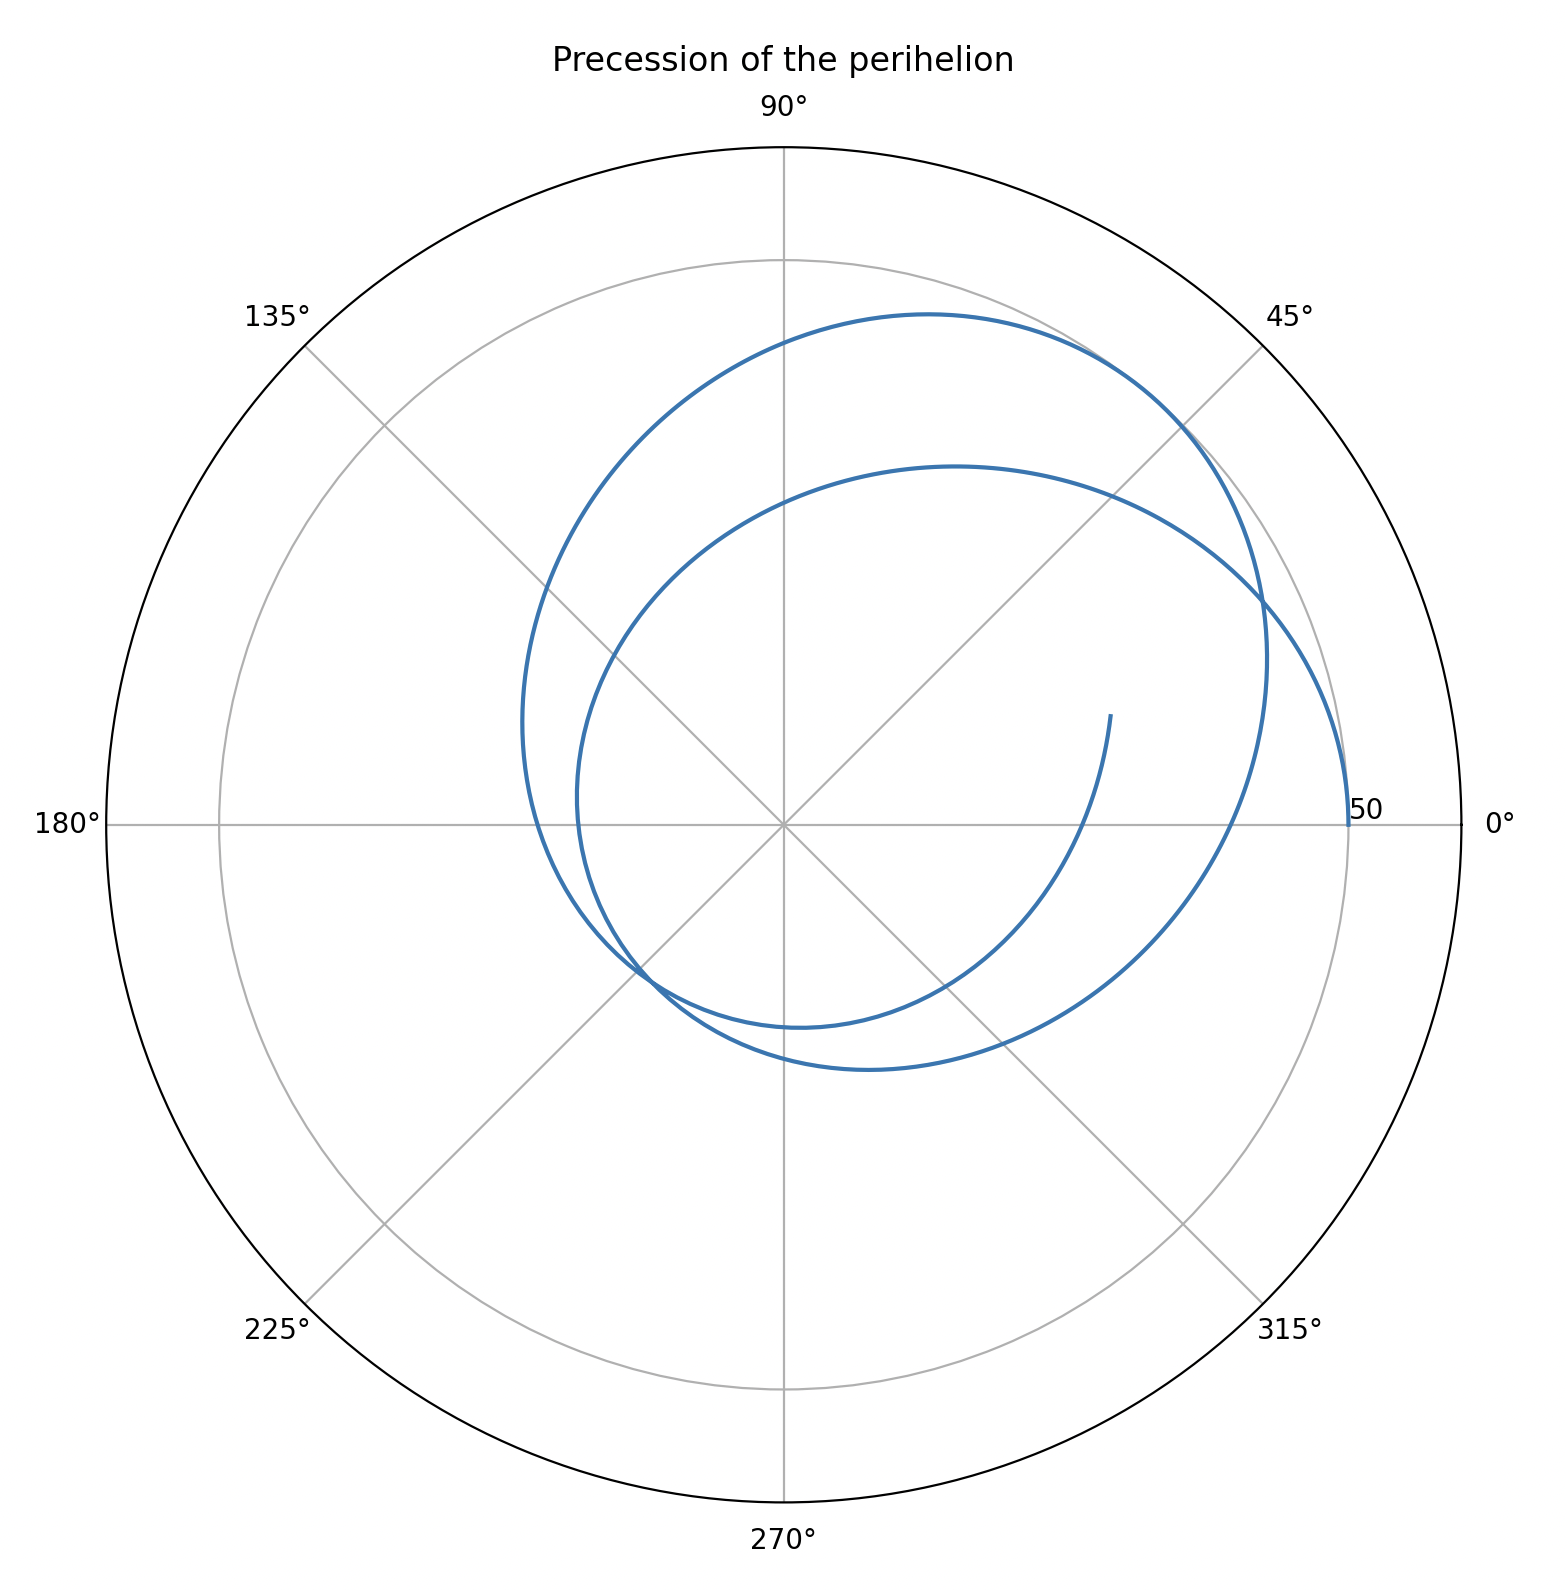
\includegraphics[scale=0.4]{ch11-p11.11.png}
    \end{center}
    Generated using \verb|ch11-p11.11.py| file.
\end{proof}

\end{document}